\documentclass{article}
\pagestyle{plain}

\usepackage{indentfirst}
\usepackage{CJK}
\usepackage{graphicx}

\begin{CJK}{UTF8}{gkai}
  \begin{document}
  \begin{center}
    \huge \bf  交通负载数据接口 项目计划
  \end{center}

  \section{项目原则}
  从善、勤奋、人性、睿智



  \section{解决的问题}
  汽车交通出行,由于无法预知行车途中车辆拥堵情况,导致大量时间、资源的浪费。



  \section{现状}
  上下班高峰期,节假日期间的高速长途出行,虽然可以通过交通频道、当地交警公示电话了解部
  分交通信息,但实时性和可信度都在问题的解决上大打折扣。
  
  目前市场上有提供实时路况功能的导航产品供消费者选择,但据考察,以下两个缺点难以克服:
  
  \begin{itemize}
  \item 价格贵

    淘宝搜索“gps 实时路况”
  \item 可用性不高

    http://gps.zol.com.cn/126/1265195.html
  \end{itemize}
  


  \section{愿景}
  该项目实施完成后,我们希望能以下场景出现在日常生活中并被大家习以为常:
  \begin{itemize}
  \item 用户在自驾由广州去武汉的途中,经过衡阳附近时,导航设备提示用户,株州段多少公里
    处塞车比较严重,建议用户前方出口下高速,改由国道行使。
  \item 用户在驾车下班途回家中,导航设备提示用户前方某个路口堵车严重,建议用户改道行驶。
  \end{itemize}
  其中,导航设备可以是目前市场上现有的车载导航仪、装有导航软件的移动智能终端等。



  \section{解决方案}
  目前市场上带实时路况功能的导航产品技术方向大致如下:

  \textbf{搜索并接受当地交通广播的路况信息(和其他交通广播信息)、解析、匹配导航线路、告警。}

  此方向虽切实可行,但其依赖的数据源依国内现有状况,无法做到行之有效。

  在此,本项目调整了技术思路,望通过如下方式解决问题:

  \textbf{提供一个可以通过互联网访问的数据接口,完成实时路况信息的查询、和更新。}

  导航设备通过互联网,或者移动互联网访问该接口,享受查询路线前方交通状况的权益,
  并承担上报已完成路线的交通状况的义务。



  \section{技术架构}
  根据以上解决方案,技术架构如图所示:
  \begin{center}
    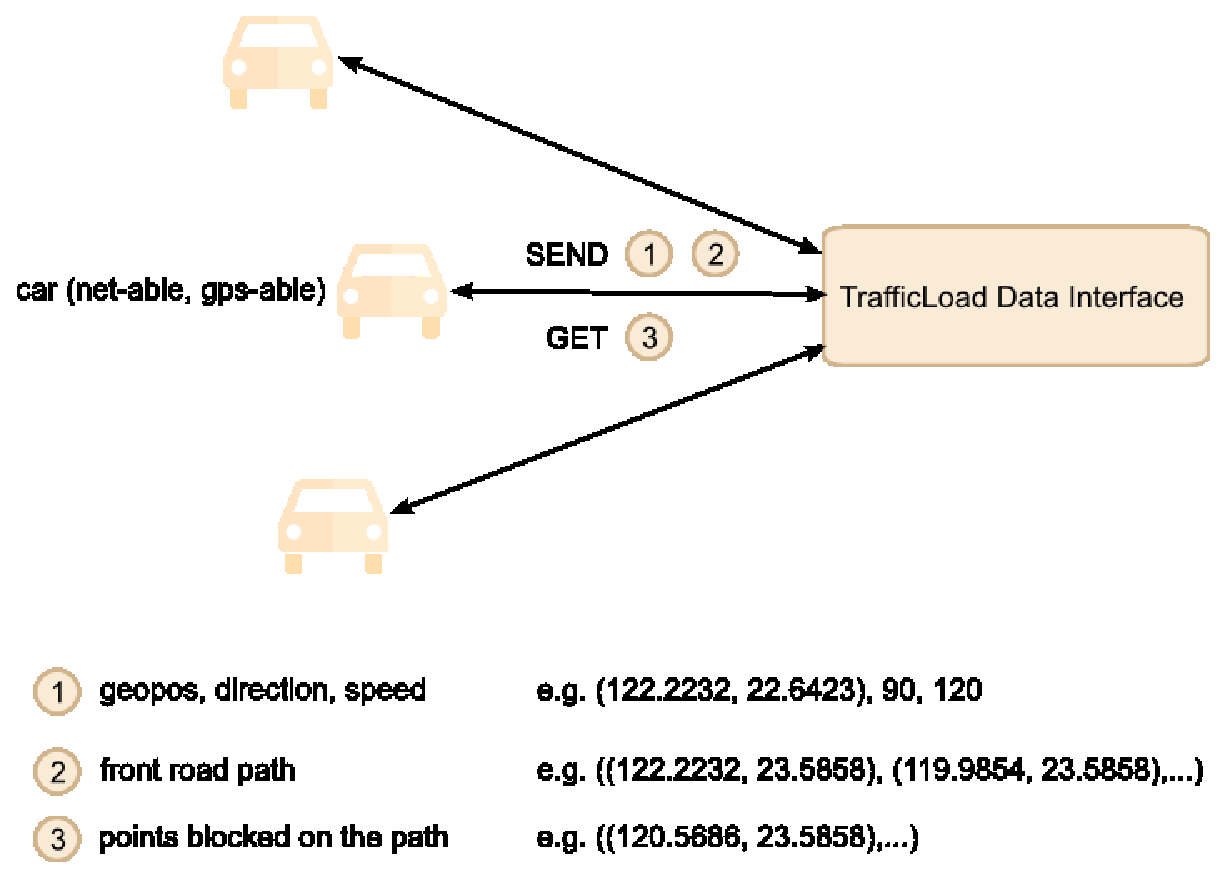
\includegraphics[width=1.2\textwidth]{tldi.eps}
  \end{center}

  \newpage
  
  看似简单的架构,却有如下几个实现难点:
  \begin{itemize}
  \item 数据的即时上报和获取

    目前,国内,能够完成任何时间,任何区域接入互联网、且具有智能处理能力的设备,只有智能手机。
    能即时准确更新车辆坐标、方向、和速度的设备只有车载gps,或者带导航功能的智能手机。
    所以,完成交通负载数据的上报和获取,需由智能手机来完成。

    虽然有车载导航的用户大部分都同时拥有智能手机,但,首先,让用户为导航设备增加到智能手机的连接,用户会稍嫌麻烦。 其次,智能手机和导航设备之间的数据传递方式有待商榷。

  \item 数据接口的性能和稳定性

    由于用户对数据的时效性和准确性要求非常高,故该数据接口需要能够快速、稳定的响应用户的请求。 特别是节假日期间,将是对系统成熟度的严峻考验。

  \end{itemize}

  另外,项目完成后,还有如下几个实施难点:
  \begin{itemize}
  \item 跨产业打通

    车载导航改造、智能手机导航改造、新增智能移动设备客户端(耗费流量上传下载)、数据接口
    都需要大量工作,每一部分都不可欠缺,需要我们慎重对待。

  \item 运营资金

    用的越多,有效性越强 是该系统的先天特征。 所以,系统开发出来以后,我们需要强有力的营销手段和资金迅速的进行推广才能确保该系统的准确性。

  \end{itemize}
  
  
  

  \section{后述}
  该项目实施起来,无论是人力还是资源上的要求都很高,困难重重。 但综合国内目前汽车、导航产品、智能移动设备的普及速度,却是切实可行、且行之有效的一套交通拥堵解决方案。

  凡能改善百姓生活的事业,必须由强烈的内心渴望、和一丝不苟的务实态度来完成。

  此刻既然觉得该项目可行,且属兴趣领域分内之事,我们便应当努力将他实现。
  
  
\end{CJK}
\end{document}
